\documentclass[11pt]{article}

\usepackage[letterpaper,margin=0.82in]{geometry}
\usepackage{amsmath}
\usepackage{graphicx}
\usepackage{microtype}
\usepackage{siunitx}
\usepackage{booktabs}
\usepackage{xcolor}
\usepackage{xr}
\usepackage[hidelinks]{hyperref}
% Figure references.  Every figure number in this project is produced by
% \ref, never typed by hand: \ref{fig:...} for figures of this document, and
% \ref{MT-fig:...} for figures of the other one, whose labels the xr package reads
% out of its .aux.  Panel letters are appended literally, e.g.
% Figure~\ref{fig:S4}a.  `make papers` compiles si -> main -> si so both
% directions resolve on a clean tree; `make check` reports any that did not.
\externaldocument[MT-]{build/main}
\usepackage{enumitem}
\usepackage{fancyhdr}
\usepackage{caption}
\usepackage{float}
\usepackage[numbers,sort&compress]{natbib}

% Line numbers, for the reviewers' convenience.  lineno does not see amsmath's
% display environments by itself, so a numbered equation would silently break
% the count; \linenoAms wraps them in \linenomath, which is the standard fix.
\usepackage[mathlines]{lineno}
\linenumbers
\newcommand*\linenoAms[1]{%
  \expandafter\let\csname old#1\expandafter\endcsname\csname #1\endcsname
  \expandafter\let\csname oldend#1\expandafter\endcsname\csname end#1\endcsname
  \renewenvironment{#1}{\linenomath\csname old#1\endcsname}%
                       {\csname oldend#1\endcsname\endlinenomath}}
\AtBeginDocument{\linenoAms{equation}\linenoAms{equation*}%
                 \linenoAms{align}\linenoAms{align*}}

\graphicspath{{figures/}}
\sisetup{detect-all=true,range-phrase=--,range-units=single}
\setlength{\parindent}{1.4em}
\setlength{\parskip}{0.55em}
\linespread{1.06}
\setlist[itemize]{leftmargin=2.0em,itemsep=0.1em,topsep=0.2em}
\captionsetup{font=small,labelfont=bf}
\pagestyle{fancy}
\fancyhf{}
\fancyhead[L]{Supporting Information}
\fancyhead[R]{\thepage}
\renewcommand{\headrulewidth}{0.4pt}
\setlength{\headheight}{14pt}
\renewcommand{\thefigure}{S\arabic{figure}}
\renewcommand{\theequation}{S\arabic{equation}}

\newcommand{\VPAVG}{(VPAVG)$_{30}$}
\newcommand{\Ainv}{\text{\AA}$^{-1}$}

% See the matching note in main.tex: data-derived figures are drawn at exactly
% the ACS column widths and are therefore included at natural size, so the 8 pt
% lettering in the file prints at 8 pt.  The photographic PNGs (S1, Video S1
% still) are not on that grid and keep an explicit width.
\newcommand{\acsfig}[1]{\makebox[\linewidth][c]{\includegraphics{#1}}}

\begin{document}

\begin{center}
{\LARGE\bfseries Supporting Information}\\[0.5em]
{\large Reversible $\beta$-Sheet-like Ordering and XPCS-Resolved Dynamic Arrest during Elastin-like Polypeptide Phase Separation}\\[1.2em]
{\normalsize Doga Ozgulbas$^{1}$, Miaoqi Chu$^{2}$, Alex Lavens$^{1}$, Nicholas Marks$^{1}$, Ming Du$^{2}$, Xiaobing Zuo$^{2}$,\\
Michael Irvin$^{1}$, Heng Ma$^{1}$, Soenke Seifert$^{2}$, Byeongdu Lee$^{2}$, Rafael Vescovi$^{1}$, Ian Foster$^{1}$,\\
Victor Mateevitsi$^{3}$, Don Jensen Jr.$^{2}$, Arvind Ramanathan$^{1,*}$, Chase Akins$^{4}$, Gyorgy Babnigg$^{4,*}$, and Qingteng Zhang$^{2,*}$}\\[0.8em]
{\small $^{1}$Data Science and Learning Division, Argonne National Laboratory, Lemont, Illinois 60439, United States\\
$^{2}$X-ray Science Division, Argonne National Laboratory, Lemont, Illinois 60439, United States\\
$^{3}$Argonne Leadership Computing Facility, Argonne National Laboratory,\\ Lemont, Illinois 60439, United States\\
$^{4}$Biosciences Division, Argonne National Laboratory, Lemont, Illinois 60439, United States}\\[0.6em]
{\small $^{*}$ramanathana@anl.gov; gbabnigg@anl.gov; qzhang234@anl.gov}
\end{center}

% A real table of contents rather than a hand-kept list: sections have moved
% three times in revision, and a generated ToC cannot fall out of step.
% tocdepth 2 includes every subsection.
\setcounter{tocdepth}{2}
\renewcommand{\contentsname}{Supporting Information Contents}
\tableofcontents
% set off from the last section entry and styled like one, so it reads as a
% peer of the numbered sections rather than a trailing remark
\vspace{1.6em}
% endpoints of the whole figure range, not references to particular figures:
% a renumbering pass rewrote the second one, so it is pinned to the last label
\noindent\textbf{Video S1 and Figures \ref{fig:S1}--\ref{fig:S10}}

\section{Recombinant Synthesis and Purification of \texorpdfstring{\VPAVG}{(VPAVG)30}}
\label{sec:synthesis}

\subsection{Materials}
Shrimp alkaline phosphatase, PfuUltra II Fusion HS DNA polymerase, GoTaq Green Master Mix, and T4 DNA ligase with PEG4000 additive were purchased from Thermo Fisher Scientific. Exonuclease I was purchased from New England Biolabs. CircLigase ssDNA ligase was purchased from Lucigen, and KOD Hot Start DNA polymerase was purchased from Sigma-Aldrich. PCR products and plasmids were purified using Monarch PCR and DNA Cleanup kits and Monarch Plasmid Miniprep columns (New England Biolabs). DNA was recovered from agarose gels using the Monarch DNA Gel Extraction kit (New England Biolabs). Oligonucleotides and the 5$'$-phosphorylated synthetic template used for rolling-circle amplification were obtained from Integrated DNA Technologies. \textit{E. coli} BL21(DE3)-Gold cells were obtained from Stratagene.

\subsection{Gene construction}
The ELP gene was prepared by overlap-extension rolling-circle amplification (OERCA).\cite{Amiram2011-la} A single-stranded DNA template encoding five VPAVG repeats was circularized in a \SI{20}{\micro\liter} reaction containing \SI{10}{\pico\mole} template, \SI{2}{\micro\liter} of 10$\times$ CircLigase buffer, \SI{1}{\micro\liter} of \SI{1}{\milli\mole\per\liter} ATP, \SI{1}{\micro\liter} of \SI{50}{\milli\mole\per\liter} MnCl$_2$, and 100 U CircLigase. The reaction was incubated for \SI{1}{\hour} at \SI{60}{\degreeCelsius}, heat-inactivated for \SI{10}{\minute} at \SI{80}{\degreeCelsius}, purified, and treated with exonuclease I for \SI{1}{\hour} at \SI{37}{\degreeCelsius} to remove unreacted linear template.

OERCA was performed with 300 ng circular template, \SI{1.5}{\micro\liter} each of \SI{50}{\micro\mole\per\liter} primers A1 and A2 (Figure~\ref{fig:S1}a), \SI{2}{\micro\liter} of 70\% GC dNTP mix, \SI{2}{\micro\liter} of \SI{25}{\milli\mole\per\liter} MgSO$_4$, \SI{10}{\micro\liter} of 10$\times$ PfuUltra II buffer, \SI{5}{\micro\liter} DMSO, and \SI{2}{\micro\liter} PfuUltra II polymerase in a total volume of \SI{100}{\micro\liter}. Cycling consisted of \SI{2}{\minute} at \SI{95}{\degreeCelsius}; 30 cycles of \SI{20}{\second} at \SI{95}{\degreeCelsius}, \SI{20}{\second} at \SI{54}{\degreeCelsius}, and \SI{90}{\second} at \SI{72}{\degreeCelsius}; and a final \SI{10}{\minute} at \SI{72}{\degreeCelsius}. Products above approximately 1.2 kb were isolated from a 0.8\% agarose gel.

Ligation-independent cloning adapters were introduced by PCR using primers B1 and B2 (Figure~\ref{fig:S1}a), and the products were inserted into the pMCSG53 vector.\cite{Aslanidis1990-lm,Eschenfeldt2009-bi} Constructs were transformed into \textit{E. coli} BL21(DE3)-Gold, screened for soluble expression, and sequence verified by Sanger sequencing. The selected construct encodes the amino-acid sequence \texttt{MHHHHHHSSGVDLGTENLYFQSNA(VPAVG)30}, comprising a cleavable N-terminal affinity/fusion sequence followed by 30 VPAVG repeats.

\subsection{Protein expression and purification}
Fresh transformants were grown in Terrific Broth containing \SI{10}{\milli\mole\per\liter} MgSO$_4$ and \SI{300}{\micro\gram\per\milli\liter} ampicillin at \SI{37}{\degreeCelsius} to an optical density of 0.6--0.8 at 600 nm. Cultures were cooled to \SI{18}{\degreeCelsius}, induced with \SI{0.2}{\milli\mole\per\liter} IPTG, and grown overnight. Cells were harvested at $5000\times g$, resuspended in ice-cold lysis buffer (\SI{500}{\milli\mole\per\liter} NaCl, 5 vol\% glycerol, \SI{50}{\milli\mole\per\liter} HEPES at pH 8.0, \SI{20}{\milli\mole\per\liter} imidazole, and \SI{10}{\milli\mole\per\liter} 2-mercaptoethanol), treated with \SI{1}{\milli\gram\per\milli\liter} lysozyme for \SI{10}{\minute}, sonicated, and clarified at $29{,}000\times g$.\cite{Makowska-Grzyska2014-cz}

The supernatant was applied to \SI{5}{\milli\liter} IMAC Sepharose High Performance resin, washed with lysis buffer, and eluted with lysis buffer containing \SI{500}{\milli\mole\per\liter} imidazole. Purification fractions were monitored by SDS-PAGE. The purified protein was exchanged into \SI{20}{\milli\mole\per\liter} HEPES at pH 8.0, \SI{250}{\milli\mole\per\liter} NaCl, and \SI{2}{\milli\mole\per\liter} DTT and concentrated using a 10 kDa molecular-weight-cutoff centrifugal concentrator. Protein concentration was determined by direct $A_{280}$ measurement on a NanoDrop spectrophotometer using the sequence-specific molar extinction coefficient applied during sample preparation (calculated molecular weight 15{,}461~Da; $\varepsilon_{280}=1490$~M$^{-1}$\,cm$^{-1}$). The final concentration was approximately \SI{100}{\milli\gram\per\milli\liter}; samples were stored at \SI{4}{\degreeCelsius}, and freshly prepared protein was used for the X-ray measurements. The expression, solubility, and purity of the protein were evaluated by SDS-PAGE (Figure~\ref{fig:S1}b).

\section{Sample Environments and X-ray Measurement Setup}
\label{sec:setup}

\subsection{Temperature-dependent SAXS/WAXS at 12-ID-B}
Temperature-dependent SAXS/WAXS was performed at APS 12-ID-B. Two aliquots of \VPAVG{} at approximately \SI{100}{\milli\gram\per\milli\liter} in \SI{20}{\milli\mole\per\liter} HEPES (pH 8), \SI{250}{\milli\mole\per\liter} NaCl and \SI{2}{\milli\mole\per\liter} DTT, nominally the same concentration used for the 8-ID-I measurements, were sealed in \SI{2}{\milli\meter} quartz capillaries. The two beamtimes fell in different APS run cycles several months apart, and because the protein is purified fresh for each experiment, the 12-ID-B and 8-ID-I material came from separate preparations of the same construct. The aliquot designated Measurement underwent more than 10 heating/cooling cycles across the thermal transition, whereas the Reference aliquot remained refrigerated at \SI{4}{\degreeCelsius}. Both aliquots were subsequently measured at \SI{10}{\degreeCelsius} and \SI{30}{\degreeCelsius} during APS run 2021-1. The \SI{13.3}{\kilo\electronvolt} beam had an approximate size of $100\times150~\mu\mathrm{m}^{2}$ and an incident flux of approximately $5\times10^{11}$ photons s$^{-1}$. SAXS was recorded with an Eiger2 9M detector at an approximately \SI{2}{\meter} sample-to-detector distance, the same energy and camera length used for a published SAXS measurement at this beamline\cite{Xu2022-12IDB} and the same camera length as another\cite{Zheng2022-12IDB}, while WAXS was recorded with a Pilatus 300K detector at \SI{0.42}{\meter}. The Pilatus detector was mounted above the direct-beam path, allowing the transmitted beam to continue to the SAXS detector so that SAXS and WAXS were acquired simultaneously with a \SI{0.1}{\second} exposure. Buffer and capillary backgrounds were subtracted, and the SAXS and WAXS profiles were stitched over their common $Q$ interval. At each set point the capillary was held at the target temperature for at least \SI{10}{\minute} before the exposures were started, so each profile reports the structure present after at least that long at temperature rather than during the temperature change. Because the two experiments used different sample cells, thermal paths, and thermometry, and because the time spent at \SI{30}{\degreeCelsius} before each 12-ID-B exposure is known only as a lower bound, the 12-ID-B \SI{30}{\degreeCelsius} profiles are not placed on the isothermal waiting-time axis of the 8-ID-I experiment; they are used here to establish the low- and high-temperature structures and their reversibility, not the kinetics of assembly.

\subsection{Isothermal SA-XPCS at 8-ID-I}
\label{sec:isoxpcs}
SA-XPCS was performed at APS 8-ID-I. Approximately \SI{100}{\milli\gram\per\milli\liter} \VPAVG{} in the same buffer was loaded into an aluminum cell containing a \SI{3}{\milli\meter}-diameter, \SI{2}{\milli\meter}-thick liquid chamber sealed by \SI{0.127}{\milli\meter} polycarbonate windows (Figure~\ref{fig:S2}). The cell was inserted into an anodized-aluminum holder in one temperature zone of the Quantum Northwest 3$\times$3 multi-sample temperature control unit, the same stage used in Ref.~\citenum{Ozgulbas2023-oz}. Each zone is driven by a Peltier element and a resistive heater, and a calibrated resistance-temperature detector (RTD) embedded adjacent to the Peltier stage supplies the controller feedback and readout. The aluminum holder and aluminum cell provided direct conductive thermal coupling. A partially coherent \SI{10.91}{\kilo\electronvolt} X-ray beam with 0.03\% FWHM bandwidth and incident flux $1.2\times10^{10}$ photons s$^{-1}$ was focused to approximately $10\times10~\mu\mathrm{m}^{2}$. Coherent scattering was recorded \SI{7.8}{\meter} downstream with a Rigaku XSPA-500k photon-counting detector comprising 1024$\times$512 pixels with a \SI{76}{\micro\meter} pixel size and a \SI{320}{\micro\meter}-thick silicon sensor. The detector was operated in 2-bit mode at a \SI{50}{\kilo\hertz} frame rate; each acquisition contained 100,000 frames, corresponding to \SI{20}{\micro\second} per frame and \SI{2}{\second} total duration. The multi-tau delay list is built from the recorded \SI{20}{\micro\second} frame time, and the longest accessible delay is \SI{1.638}{\second}.\cite{Zhang2021-jl}

For the isothermal experiment, the loaded sample was first held at \SI{6}{\degreeCelsius} for more than \SI{30}{\minute}. It was then heated to \SI{20}{\degreeCelsius} at \SI{5}{\degreeCelsius\per\minute}, followed by a slower ramp from \SI{20}{\degreeCelsius} to the target temperature of \SI{30}{\degreeCelsius} at \SI{1}{\degreeCelsius\per\minute}. The two-stage protocol was used to reduce overshoot near the target temperature. The waiting time $t_w$ was set to zero when the calibrated RTD readout reached \SI{30}{\degreeCelsius}; data collected during the preceding ramps were not included in the isothermal waiting-time series. From that point the measurement simply ran. Single \SI{2}{\second} acquisitions were taken one after another for the rest of the experiment, each at a previously unexposed position on a grid of sample positions, at a cadence of roughly \SI{6.3}{\second} per acquisition once stage motion and readout are included. A single acquisition is therefore a snapshot of a fresh piece of sample at a known $t_w$, and the series steps through increasing $t_w$ at that cadence. SAXS profiles were obtained by temporal and azimuthal averaging. Each reported elapsed time is a group average, not a single acquisition: consecutive \SI{2}{\second} acquisitions were averaged in contiguous run ranges of 63--200 acquisitions after cross-correlation outlier rejection, and the quoted $t_w$ is the acquisition time of the first run in the range. The five groups analyzed for $g_2$ begin at $t_w=5039$, 5969, 6595, 7221 and \SI{7863}{\second} and hold 150, 100, 100, 100 and 63 acquisitions, spanning 15.5, 10.4, 10.4, 10.7 and \SI{6.7}{\minute}; the last is short only because the measurement ended there. The $t_w=0$ SAXS profile of Figure~\ref{MT-fig:xpcs}a averages the first 200 acquisitions, over \SI{20.8}{\minute}. Within any one group the fitted fast fraction (Section~\ref{sec:xpcsfit}) changes by less than its own group-to-group step, so this averaging does not materially broaden the correlation functions. Correlation functions were extracted at these elapsed times once the low-$Q$ intensity provided sufficient photon statistics.

\section{12-ID-B SAXS/WAXS Analysis}
\label{sec:b12}
\subsection{Background subtraction and SAXS/WAXS merging}
The beamline-reduced \texttt{.avg} files contain $Q$, $I(Q)$ and a pointwise intensity uncertainty, the counting error $\sqrt{I}$. For each aliquot and temperature the capillary-plus-buffer profile was subtracted with a scale factor $\alpha$ of 1.00 for SAXS and the empirical 0.95 used in the original WAXS reduction, and the uncertainties were propagated through that subtraction as $\sigma=\sqrt{\sigma_{\mathrm{s}}^{2}+\alpha^{2}\sigma_{\mathrm{b}}^{2}}$. The WAXS intensity and its uncertainty were then multiplied by the ratio of the mean SAXS and WAXS intensities over their common $Q$ interval, that ratio being treated as exact, and the two profiles were concatenated and sorted by $Q$.

Those propagated uncertainties enter one result. The Guinier fit of Section~\ref{sec:guinier} is weighted, each point carrying $1/\sigma_{\ln I}^{2}$ with $\sigma_{\ln I}=\sigma_I/I$, and they therefore set the quoted errors on $R_g$ and $I_0$. The low-$Q$ power-law fit and the two Gaussian peak fits are unweighted, so the exponent and the peak centers and widths do not depend on them. Neither the 0.95 nor the overlap ratio affects a reported result either: no absolute WAXS intensity is used anywhere in this work, and the centers and widths of the two peaks, and hence the $\beta$-sheet-like spacings, depend on neither.

\subsection{Low-\texorpdfstring{$Q$}{Q} power law and WAXS peak fits}
For Figure~\ref{MT-fig:static} of the main text, the low-$Q$ slope was obtained by an unweighted linear fit of $\log_{10} I$ against $\log_{10} Q$ over $0.012<Q<0.040$~\Ainv{} for the Reference aliquot at \SI{30}{\degreeCelsius}. The two WAXS features were fitted independently to a Gaussian plus linear background over $0.48<Q<1.00$ and $1.18<Q<1.70$~\Ainv, respectively. The low-$Q$ exponent is reported as an exponent and is deliberately not converted into a fractal dimension. Two conditions set out by Teixeira\cite{Teixeira1988-jac} are not met. First, a mass-fractal dimension must satisfy $D<3$, whereas the fitted 12-ID-B slopes are $-3.17$ and $-3.15$; exponents between 3 and 4 belong instead to the surface-fractal form $Q^{-(6-D_{\mathrm{s}})}$, which that reference notes is not easily distinguished from the $Q^{-4}$ of a smooth interface. Second, a fractal description is expected to hold over at least one decade in $Q$, and the fit window $0.012<Q<0.040$~\Ainv{} spans 0.52 decades. The isothermal 8-ID-I exponents, $-2.45$ to $-2.68$, do fall below 3, so the two datasets sit on opposite sides of that boundary; this is one more reason they are treated as complementary rather than as replicate measurements of one state. The reduced profiles and scripts implementing the background subtraction, overlap scaling, Guinier analysis, power-law fit, and peak fits are available in the public repository identified in Section~\ref{sec:code}.

\subsection{Low-temperature unassembled state}
\label{sec:guinier}
The Reference profile at \SI{10}{\degreeCelsius} contains a Guinier regime satisfying $Q_{\mathrm{max}}R_g=1.246$ (Figure~\ref{fig:S3}). A fit of $\ln I(Q)$ against $Q^2$, weighted by those propagated uncertainties, gives
\begin{equation}
 R_g=22.65\pm0.50~\text{\AA}.
 \end{equation}
For reference, the cross-$\beta$ pattern is reported at approximately 4.7--4.8~\AA{} along the fibril direction and between 8 and 11~\AA{} perpendicular to it.\cite{Sunde1997-jmb,Sawaya2007-nature} Our 8.8~\AA{} falls inside that second range and our 4.5~\AA{} sits just below the first.

The fitted size is molecular in scale and is consistent with a dispersed, unassembled low-temperature state rather than persistent mesoscale aggregates. Because the protein concentration is high, this value is reported as an apparent $R_g$; weak intermolecular structure-factor contributions cannot be excluded. Recovery of the same low-temperature profile after repeated cycling establishes that the large high-temperature assembly is no longer detectable after cooling.

\section{8-ID-I Isothermal SAXS}
\label{sec:b8saxs}
\subsection{Absolute scattering cross section}
For the 8-ID-I data, the differential scattering cross section was calculated as
\begin{equation}
 I(Q)=A_s I_s(Q)-A_b I_b(Q),
 \end{equation}
where $I_s(Q)$ and $I_b(Q)$ are the temporal-mean detector intensities from the sample and buffer, per pixel and per frame. The conversion factors were
\begin{equation}
 A_j=\frac{N_{\mathrm{f}}}{F_jT_jt_{\mathrm{exp}}L\Delta\Omega},\qquad j\in\{s,b\},
 \end{equation}
where $F_j$ is the incident photon flux, $T_j$ is the transmission, $N_{\mathrm{f}}=100{,}000$ is the number of frames, $t_{\mathrm{exp}}=\SI{2}{\second}$ is the total exposure time, so that $t_{\mathrm{exp}}/N_{\mathrm{f}}$ is the \SI{20}{\micro\second} frame time, $L=\SI{2}{\milli\meter}$ is the sample thickness, and $\Delta\Omega=(d_{\mathrm{pix}}/D)^2$ is the solid angle per detector pixel.\cite{Sheyfer2020-yb} Lengths are carried in millimeters throughout, so $A_jI_j$ is in mm$^{-1}$, and that is the quantity plotted in Figures~\ref{MT-fig:xpcs}a, \ref{fig:S4}b and \ref{fig:S5}: no further scaling of any kind is applied between the calibration and the figure.

\subsection{Transmission and incident-flux calibration}
Sample transmission was obtained from ion chambers immediately upstream and downstream of the sample. Across the attenuation series, the transmission of the intervening air path was independent of beam intensity within uncertainty, with a mean value of $0.8679\pm0.0009$ (Figure~\ref{fig:S6}a; mean $\pm$ standard deviation). The upstream ion-chamber signal was converted to incident photon flux by calibration against a PIN diode positioned in the flight path upstream of the beamstop. The measured photon flux varied linearly with the upstream ion-chamber readout (Figure~\ref{fig:S6}b). The absolute-scale SAXS evolution in Figure~\ref{fig:S5} used this transmission and flux calibration.

\subsection{Isothermal SAXS evolution at \SI{30}{\degreeCelsius}}
Figure~\ref{fig:S5} shows the full SAXS sequence. At $t_w=0$, the profile is close to the \SI{6}{\degreeCelsius} reference. The low-$Q$ intensity then increases continuously and ultimately by more than two orders of magnitude, documenting progressive growth of mesoscale density contrast. The profile remains broad throughout, consistent with hierarchical network development rather than selection of a narrow domain spacing. The most pronounced increase occurs between $t_w=4088$ and 5039~s, after which the intensity continues to grow through 7863~s. This growth is what eventually brings the low-$Q$ coherent intensity above the level at which a two-step correlation function can be resolved, and is therefore the origin of the $t_w\ge5039$~s restriction. The correlation analysis in Figure~\ref{MT-fig:xpcs} of the main text uses $t_w=5039$--7863~s; earlier scattering was insufficient for reliable two-step correlations at the \SI{20}{\micro\second} frame time. The interval common to both beamlines is $0.012<Q<0.033$~\Ainv, narrower at the top end than the $0.012<Q<0.040$~\Ainv{} range behind the slopes quoted in the main text. Over that common interval the 12-ID-B \SI{30}{\degreeCelsius} profiles give power-law slopes of $-3.09$ (Reference) and $-3.07$ (Measurement), whereas the isothermal 8-ID-I series steepens from $-1.07$ at $t_w=0$ through $-1.78$ at 4088~s to $-2.45$ at 5039~s, and then stops. The last four groups give $-2.675$, $-2.670$, $-2.642$ and $-2.644$, a spread of 0.03 across the final \SI{1894}{\second}, against a step of 0.23 in the interval immediately before. Over those same \SI{32}{\minute} the intensity averaged over $0.004<Q<0.008$~\Ainv{} still grows by a factor of 1.7, so the low-$Q$ scattering keeps gaining amplitude at an essentially fixed shape. Within the window measured, then, the isothermal series is not simply en route to the 12-ID-B exponent: its shape stopped evolving about half an hour before the series ended, roughly 0.4 short of $-3.08$. The two datasets are therefore treated as complementary rather than as replicate measurements of one state, and the gap between them is not ascribed to waiting time alone, the cells, thermal paths and preparations all being different.

\section{8-ID-I SA-XPCS Correlation Analysis}
\label{sec:b8xpcs}
\subsection{Correlation functions and the fitted model}
The intensity autocorrelation function was calculated with a multi-tau algorithm,
\begin{equation}
 g_2(Q,\Delta t)=\frac{\langle I(Q,t)I(Q,t+\Delta t)\rangle_t}{\langle I(Q,t)\rangle_t^2}.
 \label{eq:si-g2}
 \end{equation}
\noindent The implementation is the 8-ID-I reduction workflow; its numerical treatment of the multi-tau scheme at these frame rates is described in detail elsewhere.\cite{Zhang2021-jl,Switalski2022-jsr}

The reduction produced 27 azimuthally averaged dynamic $Q$ bins of nominal width $1.13\times10^{-3}$~\Ainv{} spanning \SIrange{0.00376}{0.03307}{} \Ainv. The five lowest bins, centered at $Q=0.00376$, 0.00489, 0.00602, 0.00714 and 0.00827~\Ainv{} and corresponding to $2\pi/Q$ of approximately 167, 128, 104, 88 and \SI{76}{\nano\meter}, are analyzed here. Both this $Q$ restriction and the restriction to $t_w\ge5039$~s are signal-to-noise limits: the scattered intensity falls by more than an order of magnitude between the lowest bin and $Q=0.00827$~\Ainv{} (Figure~\ref{fig:S5}), so above that bin the correlation function is dominated by counting noise, and before $t_w=5039$~s the low-$Q$ intensity is itself too weak to resolve the second decay step. Figure~\ref{fig:S4}c shows the still-mobile limit of that behavior directly.

The measured $g_2$ carry two decays separated by several decades in delay, and were parameterized as a sum of two stretched exponentials,
\begin{equation}
 g_2(Q,\Delta t)=1+\beta\left[
 f(Q)\exp\!\left[-\left(\frac{\Delta t}{\tau_{\mathrm{fast}}(Q)}\right)^{p_{\mathrm{fast}}}\right]
 +\left[1-f(Q)\right]\exp\!\left[-\left(\frac{\Delta t}{\tau_{\mathrm{slow}}(Q)}\right)^{p_{\mathrm{slow}}}\right]
 \right]^2.
 \label{eq:si-twomode}
 \end{equation}
This is the same functional form used for thermoreversible nanoparticle gels, where the two-step decay is fitted as a linear sum of two stretched exponential modes with complementary amplitudes $a$ and $1-a$.\cite{Bahadur2019-ln} The same two-mode decomposition, with a fast decay and a slow stretched decay whose amplitude sets the intermediate plateau, describes ergodicity breaking in aging nanoclay suspensions.\cite{Chen2020-fn} Here $f(Q)$ is the fitted fraction of fast dynamics and $1-f(Q)$ its complement, and $\tau_{\mathrm{fast}}(Q)$ and $\tau_{\mathrm{slow}}(Q)$ are effective relaxation times; these three are free at each $Q$. The Kohlrausch--Williams--Watts exponents $p_{\mathrm{fast}}$ and $p_{\mathrm{slow}}$ carry no $Q$ argument because they are shared across the five bins in the global fit, which reduces the free parameters at each elapsed time from 25 to 17. The decomposition is phenomenological: it describes the observed first decay and persistent plateau without assigning either mode to a unique molecular mechanism.

\subsection{Calibration of the speckle contrast from a static reference}
The contrast $\beta$ of Eq.~\ref{eq:si-twomode} is set by the transverse coherence of the incident beam and by the ratio of speckle size to detector pixel size. It is a property of the beamline configuration rather than of the sample state, so it is measured once and then held fixed. The measurement used a static reference, a nano-porous glass standard of \SI{10}{\nano\meter} nominal pore diameter recorded in the same configuration shortly before the isothermal series.

A static sample does not decorrelate, so $g_2(\Delta t)=1+\beta$. For each of the 27 $Q$ bins the 50 repeat acquisitions were averaged, and a constant was fitted to that average in $\log\Delta t$ by weighted least squares using the pointwise $g_2$ uncertainties; the level of the constant is $1+\beta$. The adopted value comes from $Q=0.02067$~\Ainv{} (Figure~\ref{fig:S7}a), where the fit is flat to within its own uncertainty, with a slope of $(-3.05\pm1.84)\times10^{-5}$, that is 1.7 standard deviations from zero, and a reduced $\chi^2$ of 1.02. It gives
\begin{equation}
 \beta=0.13042\pm0.00001.
 \label{eq:si-beta}
 \end{equation}
\noindent Each of the 50 repeats is separately flat at that bin, the worst returning a reduced $\chi^2$ of 1.30 against a constant, so no repeat was rejected. The quoted error is the statistical error of that single fit; the scatter of $\beta(Q)$ in Figure~\ref{fig:S7}b is the more realistic measure of how well $\beta$ is known.

Repeating the procedure bin by bin gives $\beta(Q)$ (Figure~\ref{fig:S7}b). Twenty-three of the 27 bins return a flat averaged correlation function and a usable level; four do not. $\beta$ is flat at approximately 0.132 out to $Q\approx0.021$~\Ainv{} and falls beyond it, reaching 0.106 in the outermost bin. That falloff is instrumental: the 0.03\% bandwidth transmitted by the Si(111) monochromator sets a finite longitudinal coherence length, and the path-length difference across the scattering volume grows with scattering angle, so contrast is progressively lost as $Q$ increases. The five bins analyzed for the sample all lie below that onset. Equation~\ref{eq:si-beta} is the value used throughout, with the baseline fixed at 1.

\subsection{Global fitting and uncertainties}
\label{sec:xpcsfit}
Equation~\ref{eq:si-twomode} was fitted to all five $Q$ bins of one elapsed time at once, with $p_{\mathrm{fast}}$ and $p_{\mathrm{slow}}$ shared between the bins and $f$, $\tau_{\mathrm{fast}}$ and $\tau_{\mathrm{slow}}$ free at each $Q$. Fits minimized the error-weighted residuals $[g_{2,\mathrm{model}}-g_{2,\mathrm{data}}]/\sigma_{g_2}$ with \texttt{scipy.optimize.least\_squares}, using the pointwise $g_2$ uncertainties stored in the reduced files. Bounds were wide ($0\le f\le1$, $10^{-6}\le\tau_{\mathrm{fast}}\le10$~s, $1\le\tau_{\mathrm{slow}}\le10^4$~s, $0.2\le p\le3$) and only $f$ reaches one, refining to zero at the lowest $Q$ of the final group. The five global fits give reduced $\chi^2=0.78$--1.89. Starting values and the remaining numerical settings are in the code (Section~\ref{sec:code}).

Parameter uncertainties are the square roots of the diagonal of the covariance matrix, estimated as the Moore--Penrose pseudo-inverse of $J^{\mathrm{T}}J$ with $J$ the Jacobian of the error-weighted residuals at the solution; the pseudo-inverse is used so that a parameter refining to a bound does not leave the uncertainties of the remaining, well-constrained parameters undefined. These are the error bars plotted in Figure~\ref{MT-fig:xpcs}c. The significance of the $Q$ dependence of $f$ follows from them, the difference between two bins being compared with $\sigma=\sqrt{\sigma_i^2+\sigma_j^2}$: for adjacent bins at $t_w=5039$~s the four differences are 2.0, 2.2, 2.9 and 1.8$\sigma$, and at the four later times the smallest adjacent difference is 8.6, 11.4, 13.3 and 10.8$\sigma$. Taken end to end across the five bins the difference is 9.0$\sigma$ or more at every elapsed time. Power-law relations $\tau=AQ^{\gamma}$ in Figure~\ref{fig:S8} were obtained by weighted linear regression of $\ln\tau$ against $\ln Q$, with $\sigma_{\ln\tau}=\sigma_{\tau}/\tau$.

The slow component remains only partially relaxed during the \SI{2}{\second} acquisition and frequently yields $\tau_{\mathrm{slow}}>2$~s, so it is an effective extrapolation rather than a sampled terminal relaxation time. Conclusions about arrest therefore rest on directly observed features: the decreasing amplitude of the first decay, the rising plateau, and the systematic decrease in $f$. XPCS does not determine where the arrested regions are, $1-f$ is not a geometric volume fraction because scattering contributions are weighted by structure and contrast, and because the measurement does not reach infinite delay it is not the formal nonergodicity factor either. Figure~\ref{fig:S8} reports all auxiliary fit parameters, and Figure~\ref{fig:S9} the correlation functions and fits at the four additional $Q$ values: the same two-step shape and the same monotonic loss of the fast step appear at every measured $Q$, so the trend of Figure~\ref{MT-fig:xpcs}c belongs to the whole \SIrange{76}{167}{\nano\meter} range and not to a single bin.

\subsection{Length-scale-dependent relaxation parameters}
Figure~\ref{fig:S8} shows parameters from the global fits. Both shared stretching exponents remain below unity: $p_{\mathrm{fast}}\approx0.36$--0.70 and $p_{\mathrm{slow}}\approx0.26$--0.57. These stretched decays indicate a broad distribution of relaxation times rather than a single process. Heterogeneous, nonequilibrium dynamics of this kind are characteristic of protein and colloidal gels,\cite{Begam2021-fh,Bahadur2019-ln} although the direction of the departure from $p=1$ varies between systems: the egg-white gel of Ref.~\citenum{Begam2021-fh} relaxes with compressed rather than stretched exponentials, the signature of stress-driven rather than diffusive relaxation. The stretching found here is consistent with the approximately diffusive $\gamma_{\mathrm{fast}}\approx-2$ reported below.

The effective fast relaxation occurs on approximately $1\times10^{-4}$--$2\times10^{-3}$~s and generally becomes faster with increasing $Q$. At each elapsed time, the $Q$ dependence was parameterized as $\tau(Q)\propto Q^{\gamma}$. The fast-mode exponent is close to $-2$ at every analyzed elapsed time, $\gamma_{\mathrm{fast}}=-2.0$ to $-2.4$. At the final elapsed time the fast amplitude at the lowest $Q$ bin refines to $f=0.000\pm0.003$, i.e.\ no fast mode is detected there and $\tau_{\mathrm{fast}}$ is undefined; that bin is therefore excluded from the fast-mode panel of Figure~\ref{fig:S8} and from the corresponding power-law fit, which is why the final $\gamma_{\mathrm{fast}}$ carries a larger uncertainty. The fitted slow component also decreases with $Q$, but its tens-to-thousands-of-seconds values exceed the acquisition window; neither $\tau_{\mathrm{slow}}$ nor $\gamma_{\mathrm{slow}}$ is interpreted as a directly measured terminal relaxation law. The robust arrest measure remains the monotonic decrease in the fitted fast fraction $f$ across all five $Q$ values, equivalently the increase in the fitted slow fraction $1-f$.

\section{Radiation-Damage Mitigation and Controls}
\label{sec:radiation}
\subsection{Fresh sample positions}
The grid of positions referred to in Section~\ref{sec:isoxpcs} was Cartesian, $100\times100$ points in the aluminum cell, with adjacent points separated by at least one beam diameter. Because no position was visited twice, cumulative dose cannot track the elapsed time of the isothermal experiment, so the trend in the fitted fast fraction cannot be a dose artifact.

\subsection{Flux-dependence control}
In addition, to show that there is no significant radiation-induced artifact, an independent dose-rate test was performed after the APS Upgrade using a \SI{20}{\milli\gram\per\milli\liter} \VPAVG{} sample. Every acquisition was taken at a stage-RTD readout of \SI{33.0}{\degreeCelsius}, above the transition temperature, so the control probed the assembled high-temperature state rather than the low-temperature dispersed one. Attenuation selected incident fluxes from $2.7\times10^{11}$ to $4.9\times10^{11}$ photons s$^{-1}$, approximately 23--41 times the flux used for the main experiment. The SAXS line shapes and $g_2$ decays showed no systematic flux dependence (Figure~\ref{fig:S10}).

\section{Macroscopic and Mesoscale Structural Reversibility}
\label{sec:results}
\subsection{Macroscopic reversibility}
Video~S1 provides a direct visual demonstration of thermal reversibility. Brief warming of a capillary containing \VPAVG{} produces turbidity within approximately \SI{5}{\second}, indicating structures large enough to scatter visible light. After removal of the heat source, the sample returns to optical transparency in approximately \SI{60}{\second}. This recovery is consistent with the overlap of the cycled Measurement and refrigerated Reference SAXS/WAXS profiles at \SI{10}{\degreeCelsius}. Optical transparency does not specify molecular structure, but independently confirms dissolution of the mesoscale assembly on cooling.

\subsection{The seven-cycle experiment}
\label{sec:thermalcycling}
The reversibility comparison of Figure~\ref{MT-fig:static} sets two separate 12-ID-B aliquots against each other. The test in Figure~\ref{fig:S4} is more direct: one aliquot at 8-ID-I, taken through seven consecutive cycles and compared with itself, so that any difference between cycles can only be irreversibility. The aliquot is not the loading used for the isothermal experiment, but comes from the same stock and was measured two days apart in the same cell position of the same holder, with the cell reloaded in between. Each cycle held the sample at \SI{6}{\degreeCelsius}, ramped to \SI{34}{\degreeCelsius} at \SI{1.01}{\degreeCelsius\per\minute} over 270 consecutive \SI{2}{\second} acquisitions, and returned to \SI{6}{\degreeCelsius}, taking \SI{5.8}{\hour} in total. No acquisitions were taken during cooling, so the cooling segments of Figure~\ref{fig:S4}a are a projection from the fixed control protocol rather than a measurement; every solid segment is measured, once per acquisition, from the RTD of the stage zone holding the cell.

\subsection{Cycle-to-cycle repeatability}
Three states are sampled in every cycle: \SI{6}{\degreeCelsius}, and two windows near the top of each ramp at \SI{31.9}{\degreeCelsius} and \SI{33.8}{\degreeCelsius}. Averaged over $0.004<Q<0.008$~\Ainv, the seven cycles agree to a relative standard deviation of 9\% at \SI{6}{\degreeCelsius} and 5\% at \SI{33.8}{\degreeCelsius}, with no drift from the first cycle to the seventh. At \SI{31.9}{\degreeCelsius} the spread is 33\%, but that reflects where on the ramp each cycle happened to be sampled rather than a difference between cycles: the windows fall between \SI{31.62}{\degreeCelsius} and \SI{32.48}{\degreeCelsius}, which is on the steep part of the transition. Regressing the band-averaged $\ln I$ of each cycle on that cycle's mean window temperature gives $\mathrm{d}\ln I/\mathrm{d}T=\SI{0.95}{\per\degreeCelsius}$ with $r=0.974$, and the spread taken about that line falls to 7\%. The same regression at \SI{33.8}{\degreeCelsius}, past the steep part, takes 5\% to 1\%. The cycles therefore repeat to better than 10\% at every state once the sampling temperature is accounted for.

\subsection{Dynamics at the cycled states}
The correlation functions say what state the sample was in when each was taken (Figure~\ref{fig:S4}c). At \SI{33.8}{\degreeCelsius}, $g_2$ is flat at $1+\beta$ across the whole accessible delay range in every one of the seven cycles: the sample gelled on every heating, and the contrast measured independently on the static reference is confirmed here on the sample itself. At \SI{31.9}{\degreeCelsius} the correlation decays essentially to the baseline in the same window, so the assembly is still mobile a degree and a half lower. That is the direct evidence behind the elapsed-time restriction used in the main text: while the sample is still mobile the low-$Q$ correlation completes a single decay inside the window, leaving no second step to resolve. No correlation function is shown at \SI{6}{\degreeCelsius}, where the coherent signal at the lowest $Q$ is too weak for any contrast to be resolved.

\subsection{Cold-state artifacts and the outlier cut}
Two features of the \SI{6}{\degreeCelsius} state need comment. First, its profile still rises toward low $Q$ instead of reaching the flat Guinier plateau of a fully dispersed solution, and this is not mis-subtracted solvent: the buffer contributes only about 35\% of the signal at the lowest $Q$, so rescaling it to remove the rise would subtract most of the low-$Q$ signal and would degrade the cycle-to-cycle agreement rather than improve it. Second, the cold state is where transient scatterers appear. Taking every acquisition as recorded, the intensity at $Q=0.0035$~\Ainv{} within a single \SI{6}{\degreeCelsius} group is strongly right-skewed, while the same acquisitions at $Q=0.03$~\Ainv{} are symmetric at ordinary counting statistics; a long positive tail confined to low $Q$ is the signature of a large object crossing the $10\times10~\mu\mathrm{m}^{2}$ beam during a minority of acquisitions. The cross-correlation cut does not catch them, because it compares curve shape over the whole $Q$ range and a curve anomalous in three low-$Q$ bins alone stays close to the group mean by that measure.

A second, robust cut removes them, and is applied to every group in the paper on identical terms with no per-group list. For each acquisition the mean of $I(Q)$ over $0.004<Q<0.008$~\Ainv{} is compared with the group median, and the acquisition is rejected if it exceeds the median by more than three robust standard deviations, the scale being $1.4826\times$ the median absolute deviation and both statistics iterated to convergence. The test is one-sided because a transient scatterer only adds intensity. It removes 35 of the 1708 acquisitions surviving the cross-correlation cut, 2.0\%: 4, 2, 1, 11, 4, 1 and 1 from the seven \SI{6}{\degreeCelsius} groups, 2 and 7 from the two buffer groups, and none at all from any of the fourteen high-temperature windows, which is consistent with the skew being confined to the cold state. Elsewhere it is nearly inert, removing two acquisitions of the isothermal series, shifting one absolute-scale coefficient by 0.03\% and leaving every fitted correlation-function parameter unchanged. Its effect here is reported rather than absorbed: the cycle-to-cycle spread at \SI{6}{\degreeCelsius} falls from 13\% to 9\%, and what remains is a mild rise over the last two cycles rather than one anomalous group. The threshold is not tuned, the same acquisitions being selected for any value between 2.5 and 3 and for two other choices of band.

One difference between the two loadings survives all of this and is a property of the material rather than of a few acquisitions: the cycling loading has $I(0.004)/I(0.02)=4.0$ against 2.7 for the isothermal loading, and transmits 0.305 against 0.333. It was the less completely dissolved of the two.

\section{Code, Data and AI-Assisted Development}
\label{sec:code}
\subsection{Code and reduced-data availability}
\label{sec:availability}
The reduced datasets and all analysis and figure-generation code used for this manuscript are publicly available at \url{https://github.com/qzhang234/PubCode-2021-IDPP}. The repository includes the reduced 12-ID-B SAXS/WAXS data, the averaged 8-ID-I XPCS HDF files for every group plotted, the per-acquisition temperature record of the thermal-cycling sequence, the individual correlation functions of the speckle-contrast standard, radiation-control data, absolute-intensity calibration inputs, and the scripts used to generate the main-text and Supporting Information figures. Every data-derived figure can be regenerated from the repository alone. Two further scripts document how the committed reduced files were produced from the raw beamline results. \texttt{SAXS\_12id/Read\_12ID\_SAWAXS.py} handles 12-ID-B, merging the SAXS and WAXS profiles into the committed CSV files. \texttt{SAXPCS\_8id/average\_ranges.py} handles 8-ID-I, applying both outlier-rejection passes to every group on the same terms and averaging each into the committed HDF files. Both read the beamline storage directly. The repository README maps each script and output file to the corresponding manuscript figure. The repository carries the reduced data rather than the raw detector frames, for two reasons. The first is volume. Every \SI{2}{\second} acquisition is 100,000 detector frames, and the isothermal and thermal-cycling series together run to several thousand acquisitions, which puts the raw dataset orders of magnitude beyond the roughly 150~MB of reduced data committed here. The second is where the archival copy lives: Advanced Photon Source project storage, which is reachable only from machines inside the facility network. Raw data are available from the corresponding authors.

\subsection{AI-assisted development}
\label{sec:ai}
The authors used Claude Sonnet 5 and Opus 5 to assist with the manuscript preparation and code development. The Claude models were accessed through Argo, Argonne National Laboratory's internal generative AI interface, which provides Laboratory staff with access to large language models from multiple vendors, including Anthropic, OpenAI, and Google, for use in Laboratory research and operations. 

Qingteng Zhang reviewed the code, reran the analyses, and confirmed the reported results. The code is public (Section~\ref{sec:availability}), so every reported number and data-derived figure can be checked independently. All analysis choices, scientific interpretations, and manuscript content were determined by the authors, who take full responsibility for the publication.

\clearpage
\section*{Supporting Video}
\begin{center}
  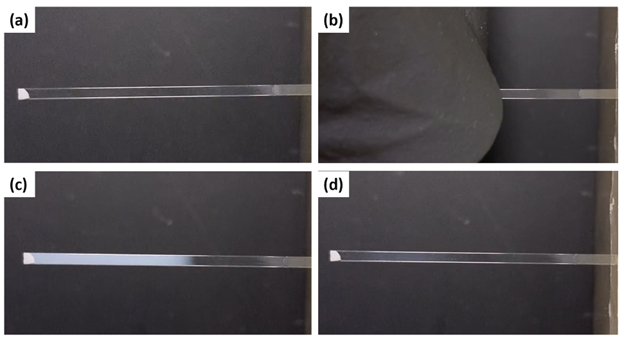
\includegraphics[width=0.88\linewidth]{VideoS1_Still.png}
\end{center}
\textbf{Video S1. Reversible thermal transition in \VPAVG.} (a) A thin quartz capillary containing \VPAVG{} is held in a fixture. (b) The capillary is warmed for approximately \SI{5}{\second} by contact through nitrile gloves. (c) The initially transparent solution becomes visibly turbid. (d) The sample returns to transparency approximately \SI{60}{\second} after removal of the heat source. The complete video can be viewed or downloaded at \url{https://anl.app.box.com/s/lsukldjnr45nhfrkobijsar1tqhba7jw}.

\clearpage
\begin{figure}[H]
\centering
{\raggedright\textbf{(a)}\par}
\vspace{0.2em}
\fbox{\begin{minipage}{0.90\linewidth}
\raggedright\ttfamily\small
\textbf{A1 (forward)}\\
5$'$-GTTCCAGCTGTTGGTG\\[0.5em]
\textbf{A2 (reverse)}\\
5$'$-ACCTACTGCTGGTACG\\[0.5em]
\textbf{B1 (forward)}\\
5$'$-TACTTCCAATCCAATGCCGTTCCAGCTGTTGGTGTGCCG\\[0.5em]
\textbf{B2 (reverse)}\\
5$'$-TTATCCACTTCCAATGTTAACCTACTGCTGGTACGCCGAC\\[0.5em]
\textbf{VPAVG$_{30}$ OERCA single-stranded template}\\
/5Phos/GTTCCAGCTGTTGGTGTGCCGGCCGTGGGCGTGCCTGC\\
GGTGGGCGTCCCGGCGGTCGGCGTACCAGCAGTAGGT
\end{minipage}}

\vspace{1.4em}
{\raggedright\textbf{(b)}\par}
\vspace{0.2em}
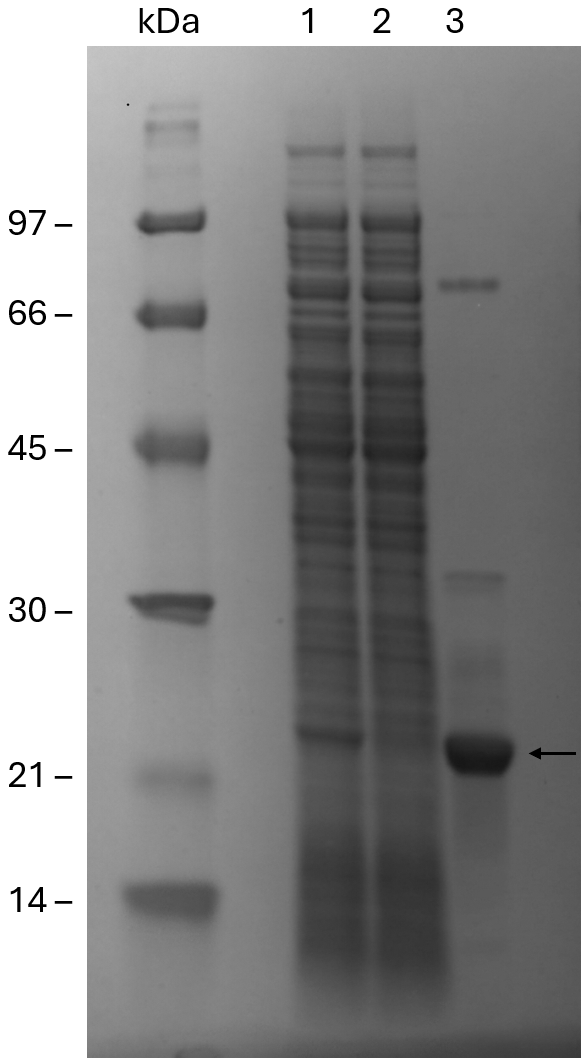
\includegraphics[width=0.34\linewidth]{FigureS1b_SDS_PAGE.png}
\caption{Construction and expression of the \VPAVG{} gene. (a) Oligonucleotide primers and the 5$'$-phosphorylated single-stranded OERCA template used to construct the ELP gene. (b) SDS-PAGE analysis of expression and purification. Samples were resolved by SDS-PAGE and stained to evaluate expression, solubility, and purity of the heterologously expressed protein. The molecular-weight marker lane is at the left, with prominent bands labeled in kilodaltons (kDa). Lanes 1--3 are the total soluble fraction, the flow-through fraction after IMAC, and the eluted fraction, respectively. The arrow marks the eluted \VPAVG{} construct, whose apparent mobility is lower than that expected from its calculated mass of 15{,}461~Da.}
\label{fig:S1}
\end{figure}
\clearpage
\begin{figure}[H]
  \centering
  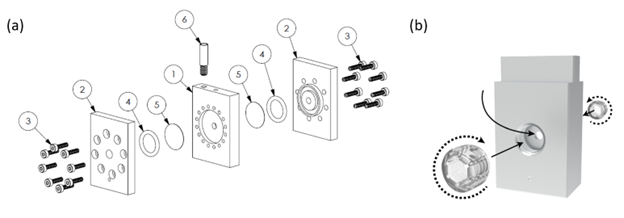
\includegraphics[width=0.94\linewidth]{FigureS2_Sample_Cells.png}
  \caption{Sample cells used for liquid X-ray measurements. (a) Exploded view of the aluminum cell used for the 8-ID-I isothermal SA-XPCS experiment. The cylindrical chamber is \SI{3}{\milli\meter} in diameter and \SI{2}{\milli\meter} thick along the X-ray direction; \SI{0.127}{\milli\meter} polycarbonate windows are compressed by Viton O-rings and bolted caps. During measurement, this cell was inserted into the anodized-aluminum holder of the Peltier-controlled stage described in Section~\ref{sec:isoxpcs}; both the holder and cell were aluminum. (b) Screw-cap cell developed separately for automated handling; the dashed circles magnify the window seat. Only the bolted aluminum cell in panel (a) was used for measurements reported in the main text. The circled numerals in (a) identify the components: (1) the aluminum cell body, which contains the sample chamber; (2) the aluminum cap plates; (3) M2 screws, \SI{8}{\milli\meter} long, which clamp the caps against the body; (4) Viton O-rings; (5) window disks cut from Kapton or polycarbonate sheet with a hammer-driven punch, polycarbonate being used for the measurements reported here; and (6) the handle used to withdraw the cell from the Quantum Northwest stage. Labels (2)--(5) appear on both sides of the body because the assembly is symmetric about the sample chamber.}
  \label{fig:S2}
\end{figure}
\clearpage
\begin{figure}[H]
  \centering
  \acsfig{FigureS3_Guinier.pdf}
  \caption{Guinier analysis of the Reference aliquot at \SI{10}{\degreeCelsius}. Weighted linear fit of $\ln I(Q)$ against $Q^2$ over $0.020\le Q\le0.055$~\Ainv{} (so $Q_{\mathrm{max}}R_g=1.246$), giving an apparent $R_g=22.65\pm0.50$~\AA{} and $I_0=1.725\pm0.023$ in the arbitrary intensity units of the reduced 12-ID-B profiles. Points are plotted over the wider range $0.005\le Q\le0.080$~\Ainv{} for context; error bars are the propagated intensity uncertainties, $\sigma_I/I$.}
  \label{fig:S3}
\end{figure}
\clearpage
\begin{figure}[H]
  \centering
  \acsfig{FigureS4_Thermal_Cycle.pdf}
  \caption{Thermal-cycling repeatability of the SA-XPCS sample: one aliquot, a separate loading from the isothermal experiment of Figure~\ref{MT-fig:xpcs} of the main text, through seven consecutive cycles. (a) Sample temperature over the \SI{5.8}{\hour} sequence. Solid curves are measured: the stage RTD was read once per \SI{2}{\second} acquisition. No acquisitions were taken while the sample cooled, so no temperature was recorded over those intervals; the dashed curves there are not data but the profile projected from the control protocol, which was fixed at \SI{10}{\degreeCelsius\per\minute} cooling until \SI{6}{\degreeCelsius} followed by a hold at \SI{6}{\degreeCelsius} until the next ramp. Open symbols mark, at the time and temperature at which it was taken, every acquisition group that is plotted in (b) and (c), so each lower-panel curve can be traced to its point in the thermal history. (b) Buffer-subtracted SAXS on an absolute scale at \SI{6}{\degreeCelsius} (circles, 32--41 surviving acquisitions averaged; see Section~\ref{sec:thermalcycling}), \SI{31.9}{\degreeCelsius} (squares, acquisitions 241--250) and \SI{33.8}{\degreeCelsius} (triangles, acquisitions 261--270). Each group is placed on the absolute scale with the mean ion-chamber readings of the acquisitions it contains, and the averaged buffer (69 surviving of 89 acquisitions, D0077 and D0080) is subtracted with no empirical scale factor, exactly as in Figure~\ref{MT-fig:xpcs}a. (c) Correlation functions at the lowest $Q$ bin for the two high-temperature states; the dotted line is $1+\beta$ with $\beta$ the contrast measured in Figure~\ref{fig:S7}. Error bars are the measured pointwise $g_2$ uncertainties; the $y$ axis is capped so that a few short-delay caps clip. One key serves all three panels: its columns are the seven thermal cycles, numbered along the top and colored on the same scale Figure~\ref{MT-fig:xpcs} of the main text uses for elapsed time, and its rows are the three temperature states, labeled at the left and distinguished by marker shape.}
  \label{fig:S4}
\end{figure}
\clearpage
\begin{figure}[H]
  \centering
  \acsfig{FigureS5_SAXS_Evolution.pdf}
  \caption{Complete isothermal SAXS evolution of \VPAVG{} at \SI{30}{\degreeCelsius}, buffer-subtracted and on the same absolute scale as Figure~\ref{MT-fig:xpcs}a of the main text, using the same buffer measurement. The \SI{6}{\degreeCelsius} reference and profile at the start of the hold are followed by profiles from 1249 to 7863~s. White marks on the color bar give the elapsed time of each measured profile. Colors here are scaled linearly over the full \SIrange{0}{7863}{\second} range and therefore do not match the discrete colors used for the same times in Figure~\ref{MT-fig:xpcs}; read times from the color bar. The subset from 5039 to 7863~s corresponds to the SAXS and SA-XPCS data analyzed in Figure~\ref{MT-fig:xpcs} of the main text.}
  \label{fig:S5}
\end{figure}
\clearpage
\begin{figure}[H]
  \centering
  \acsfig{FigureS6_Calibration.pdf}
  \caption{Transmission and photon-flux calibration for conversion to absolute scattering cross section. (a) Air-path transmission across seven measurements in the attenuation series; the line marks the mean, $0.8679\pm0.0009$ (standard deviation). (b) Photon counts recorded by a calibrated PIN diode as a function of the upstream ion-chamber readout (both in the scaled detector units of the calibration series); the line is the linear calibration fit, from which the incident flux follows as $F=(A\cdot\mathrm{Up\_IC})/t_{\mathrm{exp}}+B$.}
  \label{fig:S6}
\end{figure}
\clearpage
\begin{figure}[H]
  \centering
  \acsfig{FigureS7_Contrast.pdf}
  \caption{Measurement of the instrumental speckle contrast $\beta$ on a static reference. (a) Correlation functions of a \SI{10}{\nano\meter} nano-porous glass standard at $Q=0.02067$~\Ainv, the best-counted bin whose averaged correlation function is flat to within its uncertainties: 50 individual repeat acquisitions (grey) and their average (black, with the measured pointwise uncertainties). The red line is a straight-line fit in $\log\Delta t$; it is flat to 1.7 standard deviations with reduced $\chi^2=1.02$, as a static sample requires, and its level gives $\beta=0.13042\pm0.00001$. (b) The same procedure applied bin by bin. $\beta$ is essentially independent of $Q$ across the shaded range used for the sample; the red line is the fixed value from (a). Above $Q\approx0.021$~\Ainv, outside that range, $\beta$ falls off as the finite longitudinal coherence length set by the Si(111) monochromator begins to limit the contrast. Four of the five bins used for the sample return $\beta=0.1297$, 0.1328, 0.1318 and 0.1319, all within 2\% of it. Four bins out of 27 whose averaged correlation function is not flat (reduced $\chi^2>5$, detector and parasitic-scattering artifacts) are omitted, one of them at $Q=0.00489$~\Ainv{} inside the shaded range.}
  \label{fig:S7}
\end{figure}
\clearpage
\begin{figure}[H]
  \centering
  \acsfig{FigureS8_Fit_Parameters.pdf}
  \caption{Additional parameters from global two-mode fits. Colors denote elapsed time as in Figure~\ref{MT-fig:xpcs} of the main text (5039, 5969, 6595, 7221 and 7863~s, dark to light). (a) Stretching exponents shared across the five $Q$ bins at each elapsed time. (b) Effective fast relaxation time versus $Q$. (c) Fitted scaling exponents $\gamma_{\mathrm{fast}}$ and $\gamma_{\mathrm{slow}}$. (d) Effective slow relaxation time versus $Q$. Dashed lines in panels (b,d) are power-law fits $\tau\propto Q^{\gamma}$. At the final elapsed time the fast amplitude at the lowest $Q$ bin refines to $f=0.000\pm0.003$, so no fast mode is detected there and $\tau_{\mathrm{fast}}$ is undefined; that point is omitted from (b) and from its power-law fit, which is why the final $\gamma_{\mathrm{fast}}$ has a larger uncertainty. The slow-mode quantities are extrapolations beyond the accessible delay range; $\gamma_{\mathrm{slow}}$ at the earliest elapsed time, $-3.78\pm0.37$, lies well outside the $-1.4$ to $-1.9$ spanned by the other four, and is the least constrained of the set because the slow mode carries its smallest amplitude there. Grey lines connect points belonging to the same parameter and are guides to the eye; the dotted line in (a) marks $p=1$, the simple-exponential limit. Error bars are fit uncertainties.}
  \label{fig:S8}
\end{figure}
\clearpage
\begin{figure}[H]
  \centering
  \acsfig{FigureS9_g2_Grid.pdf}
  \caption{Expansion of Figure~\ref{MT-fig:xpcs}b of the main text onto the four higher $Q$ bins. Panels show (a) $Q=0.00489$, (b) 0.00602, (c) 0.00714, and (d) 0.00827~\Ainv. Colors denote the same elapsed times as Figure~\ref{MT-fig:xpcs}b,c of the main text. Solid curves are the same global two-mode fits that produce Figure~\ref{MT-fig:xpcs}c and Figure~\ref{fig:S8}: at each elapsed time all five $Q$ bins are fitted simultaneously with $p_{\mathrm{fast}}$ and $p_{\mathrm{slow}}$ shared across $Q$ and $\beta$ fixed at the measured instrumental contrast, and the curve drawn in each panel is that global solution evaluated at that panel's $Q$. Error bars are the measured pointwise $g_2$ uncertainties. The $y$ axis is capped at 1.20; two of 1220 plotted points and four error-bar caps, all at the shortest and noisiest delays, fall above it.}
  \label{fig:S9}
\end{figure}
\clearpage
\begin{figure}[H]
  \centering
  \acsfig{FigureS10_Flux_Control.pdf}
  \caption{Flux-dependence control for SAXS and SA-XPCS. (a) SAXS profiles and (b) intensity autocorrelation functions from a \SI{20}{\milli\gram\per\milli\liter} \VPAVG{} sample at incident fluxes of $2.7\times10^{11}$--$4.9\times10^{11}$ photons s$^{-1}$. The $Q$ range shown in (a), \SIrange{0.0024}{0.051}{} \Ainv, covers the $Q$ range of Figure~\ref{MT-fig:xpcs}a of the main text. Intensities in (a) are detector counts per pixel per frame, not on the absolute scale of Figure~\ref{MT-fig:xpcs}a. Panel (b) shows the lowest $Q$ bin of this control configuration, $Q=0.00304$~\Ainv{} ($2\pi/Q\approx\SI{206}{\nano\meter}$). The legend orders the four conditions by nominal attenuator setting, which is not monotonic in flux. No systematic flux-dependent change is resolved over this range, which substantially exceeds the flux used in the main experiment.}
  \label{fig:S10}
\end{figure}
\bibliographystyle{achemso}
\bibliography{reference}

\end{document}
